\section{Euclidean distance}
Given two time-series $X=(x_{1},x_{2}...x_{n})$ and $Y=(y_{1},y_{2}...y_{m})$ where $n=m$ the Euclidean distance is defined as
\begin{equation}
 D_{euclidean}(X,Y) = \sqrt{ \sum_{i=1}^{n}  (x_{i} - y_{i})^2 }
\end{equation}
While being easiest to calculate and satisfying all the distance requirements the Euclidean distance, when applying to the raw time-series data, seems to bee too rigid to capture similarity between time series which follow the very same pattern in time but somehow different in scale. In \cite{citeulike:4107287} authors outlining that Euclidean distance is ``..impractical in several applications, particularly for multimedia applications, where shrinking and stretching of the data are very typical'' and providing an example of two time-series representing the ``Happy birthday'' tune which were found very similar after scaling and normalization \ref{fig:happybirthday}
\begin{figure}[tbp]
   \centering
   \includegraphics[height=90mm]{happy_birthday.eps}
   %%{seriesheatmap}
   \caption{a) Figure taken from \cite{citeulike:4107287} depicts raw pitch contour extracted from a sung query represents a query sequence Q, and a MIDI pitch contour of �Happy Birthday� song represents a candidate sequence C. b) A rescaled query sequence Q with scaling factor = 1.25. c) Both sequences after mean normalization at the query�s length. The shaded region shows their Euclidean distance.}
   \label{fig:happybirthday}
\end{figure} 

Therefore, in order to make an efficient application of the Euclidean distance we have to apply a normalization technique to transform time-series into the space suitable for the Euclidean-distance based comparison. The normalization techniques are the next topic of this review.